\chapter{Infrastructure}
\label{cha:infrastructure}

\section{Storing the dataset}
\label{sec:storingthedataset}
We stored the dataset in multiple ways, each better suited for different tasks.

The original WikiConv, its four sorted copies, and the relative minified versions were stored as compressed gzip files on a hard disk and backed up in Google Drive. This hard drive was accessible from all the computers we used to perform the analysis.

A copy of the original dataset was decompressed and loaded in a MongoDB instance, where the look-up table was also created. MongoDB is a non-relational database that uses a JSON structure for its data, making it a good fit for the WikiConv data structure. It was used to launch simple queries on the dataset and retrieve immediate results. MongoDB was also useful for other related projects, which used our data in their analysis, and could easily use it.

\section{Storing our results}
\label{sec:storingourresults}
Results are stored in four ways: A Postgres database,\footnote{\url{https://www.postgresql.org/}} A mongoDB instance, JSONs files and CSVs files.

Among all members of our group, we choose to use a similar format for all our metrics. All the relevant metrics we generated can be saved in a Postgres database and do not contain sensitive information. Each Table collects information about a single language analyzed. The rows every month are analyzed for each page and user group.

MongoDB was mostly used for the look-up tables. It was also used to extract the information needed during our analysis that was made by other team members and was stored on a MongoDB instance.

JSON files were used to save simple results, that could be shared or used to plot charts.

CSV files were mostly used to save data used in our analysis that did not need to be loaded to a proper database and needed to be read quickly from a file. This is also the format the emotion EmoLex used.

\section{Public API}
\label{sec:publicapi}
We want to make publicly available the metrics we calculated, but the dataset is large and, usually, only a small portion of it is necessary for any related work. Forcing people to load the whole dataset can be time-consuming and take up lots of resources, setting a high bar for anybody interested in using our data. To reduce this stress, we decided to make a public API endpoint. People can now query our dataset without the need to install it on their machine and retrieve only the information they need.

To maximize the flexibility of our APIs results, we implemented GraphQL, a query language made for APIs.\footnote{\url{https://graphql.org/}} It allows users to write and send to our backend their query. We can validate and execute their request and return the data in the format they asked for. GraphQL also offers a landing page, reachable from any browser where user can compose their query and are helped by the UI to understand our database structure.

To link GraphQL to our Postgres database we used Hasura, a software that automatically maps a Postgres database to GrapQL. This solution allowed us to use GraphQL, without the need to implement a custom backend. We configured Hasura to allow anybody to read our data, but without the possibility to alter it.\footnote{\url{https://hasura.io/}}

\begin{figure}[H]
    \centering
    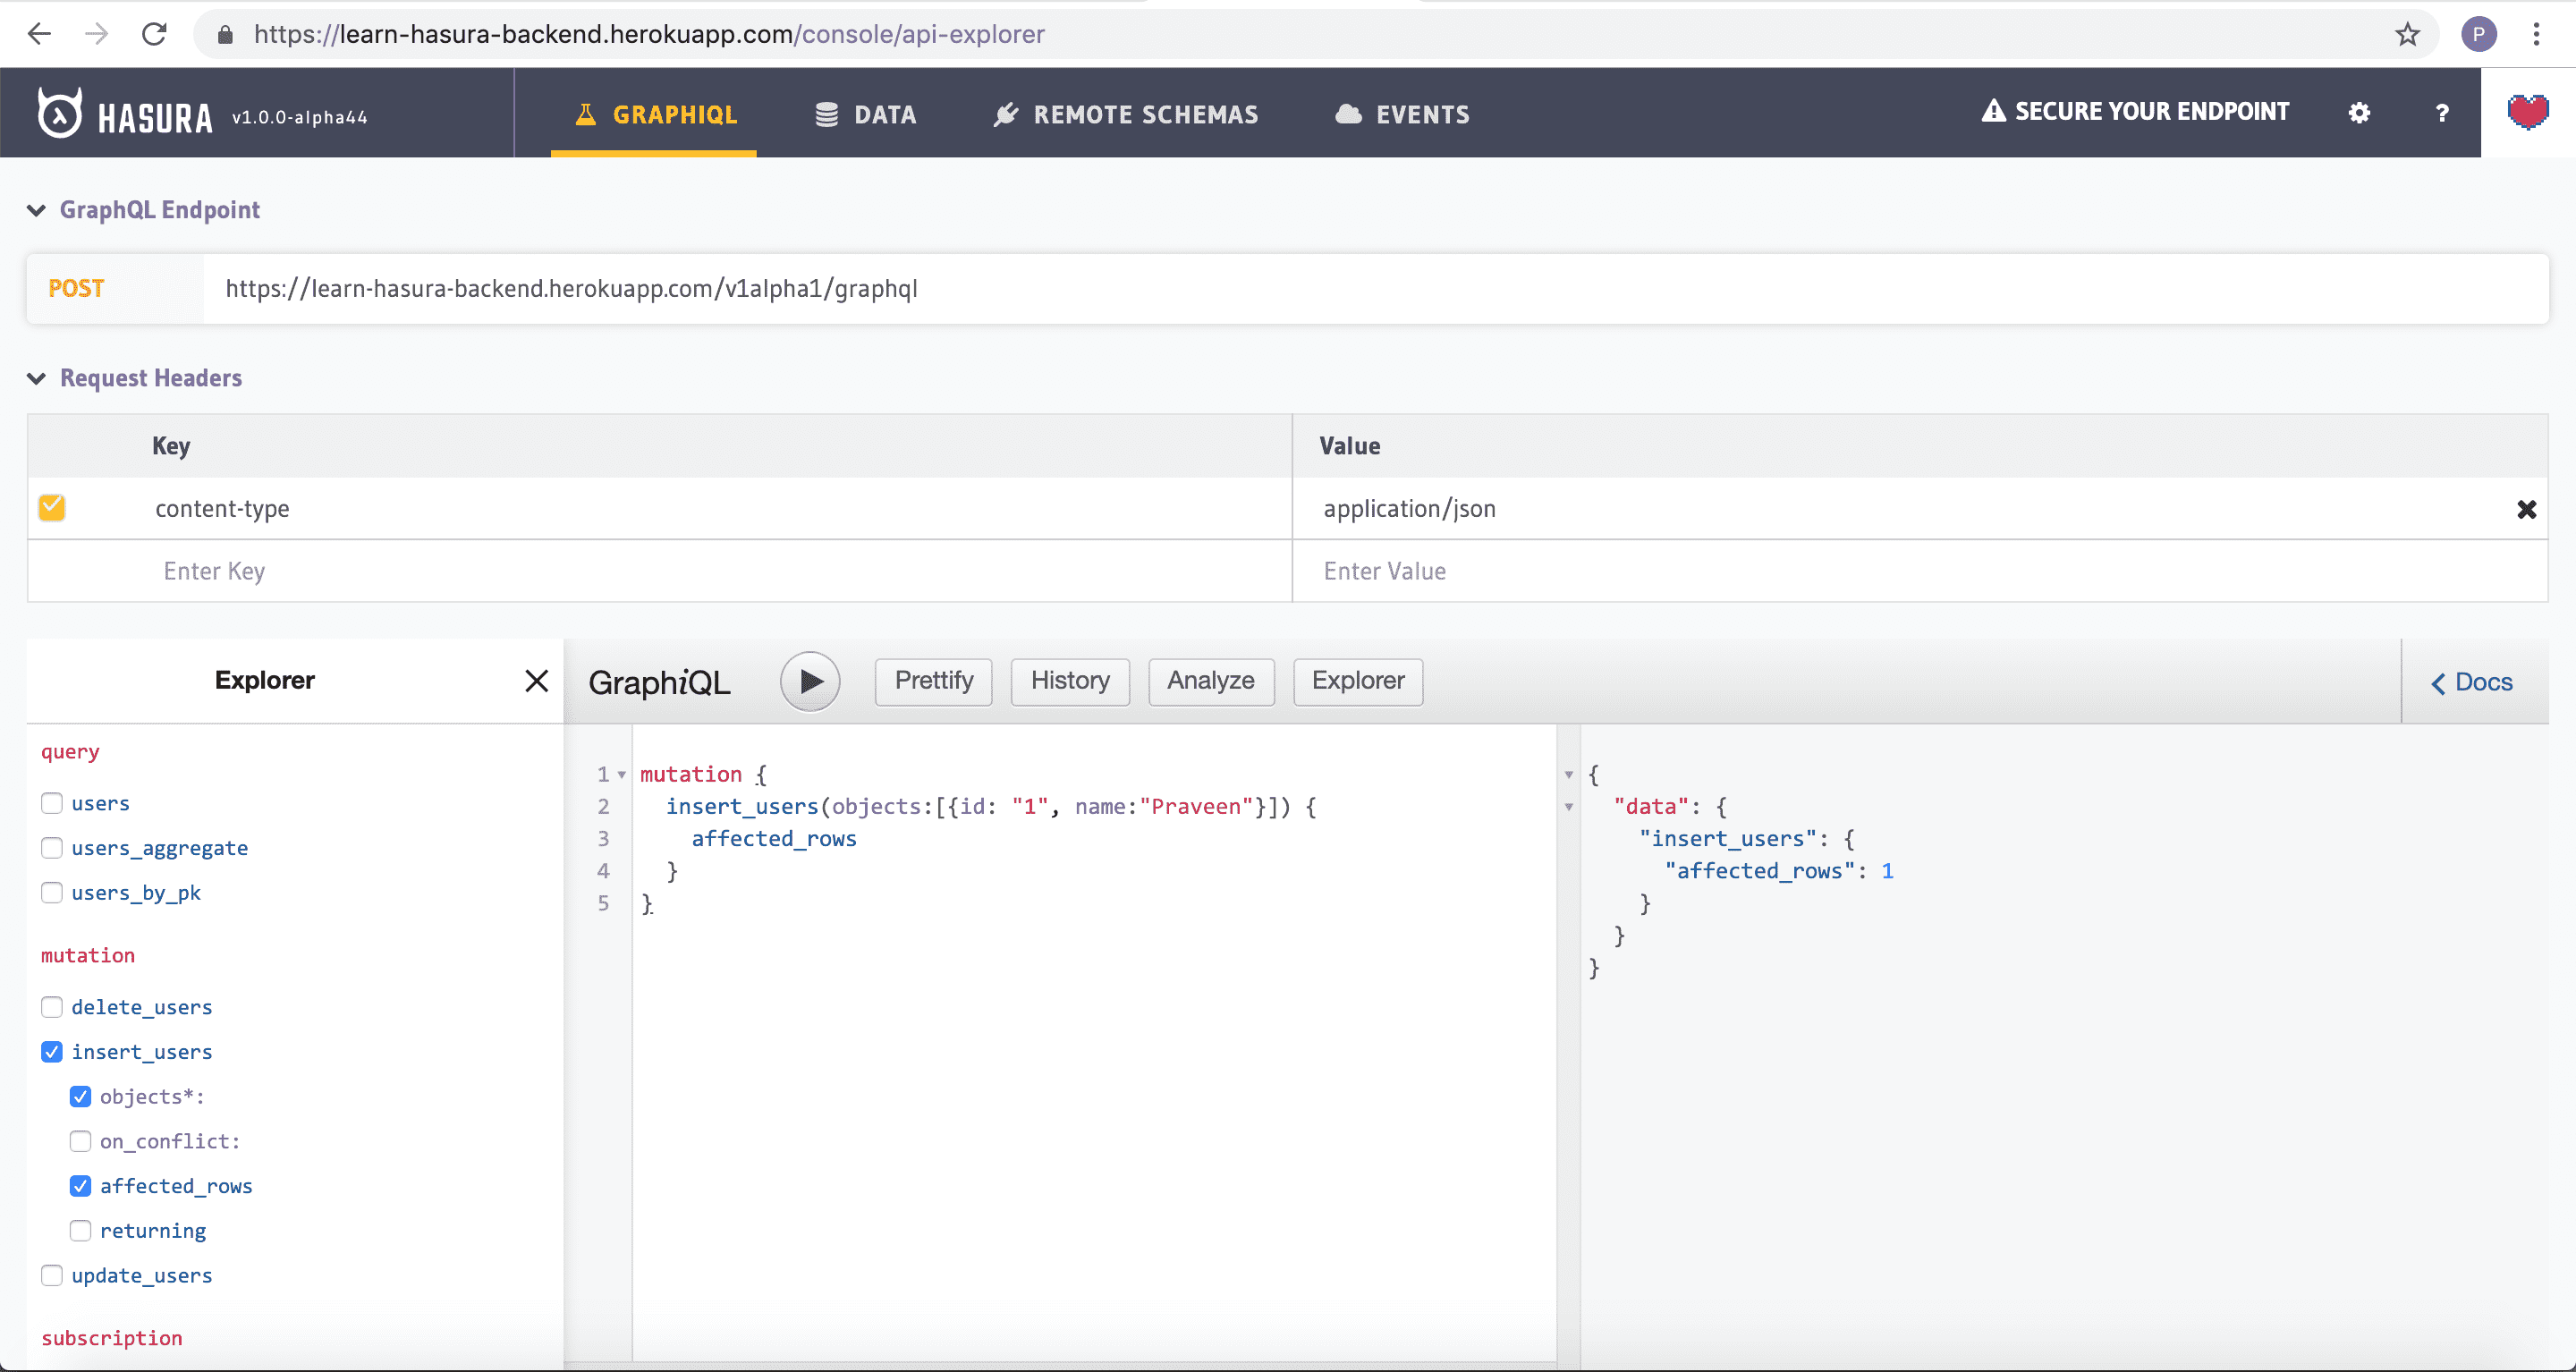
\includegraphics[width=0.8\textwidth]{./img/hasura.png}
    \caption{Hasura landing page, where a user can query our database}
    \label{fig:hasura}
\end{figure}

\section{Web Application}
\label{sec:webapplication}
We developed a web application to show chart combining multiple metrics. This application was developed in TypeScript\footnote{\url{https://www.typescriptlang.org/}} using the Vue.js framework.\footnote{\url{https://vuejs.org/}} For the charts we used the JavaScript version of Plotly.\footnote{\url{https://plotly.com/javascript/}}

The Web application provides a simple and accessible tool for anybody that wants to read and plot out metrics. It is accessible from a browser, and through a graphical user interface allows users to select which metrics to plot and compare. Thanks to the metrics being saved similarly, results from multiple projects from our team can be implemented.

The web application was developed in Typescript using Vue.js 3, a progressive JavaScript Framework. All code developed in Vue.js runs on the user browser, avoiding the need for us to maintain a complex infrastructure active, it is only required to serve the static HTML and JavaScript files from the server. To retrieve the data needed by a user, the web application queries the Hasura instance. This is done through Apollo,\footnote{\url{https://www.apollographql.com/}} a GraphQL implementation for Vue.js.

The charts were made with Plotly JavaScript, a charting library, which allows us to build complex charts with a high-level implementation. Charts show different metrics simultaneously and can be personalized by users.

\begin{figure}[H]
    \centering
    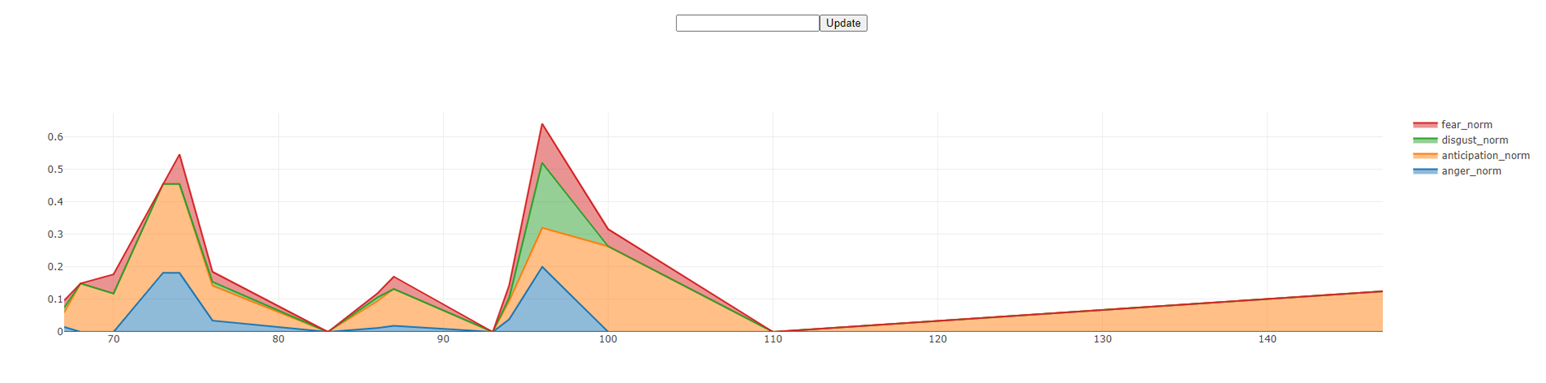
\includegraphics[width=0.95\textwidth]{./img/app.png}
    \caption{A page of the web app where a chart is showing severla metrics chosed by a user}
    \label{fig:chainsuser}
\end{figure}

\section{Deploy}
\label{sec:deploy}
To deploy our solution, we decided to use Docker.\footnote{\url{https://www.docker.com/}} It is a software that uses virtualization technology to deliver software in packages called container. Containers are isolated from one another and bundle their own software. Thanks to this technology we can deploy our database, Hasura, and our web application in three different containers. We can deploy our solution without worries about dependencies and compatibility, moreover, all our software is isolated and can be updated with continuous integration.

The Hasura container is public and anybody can implement their application using our data.

\begin{figure}[H]
    \centering
    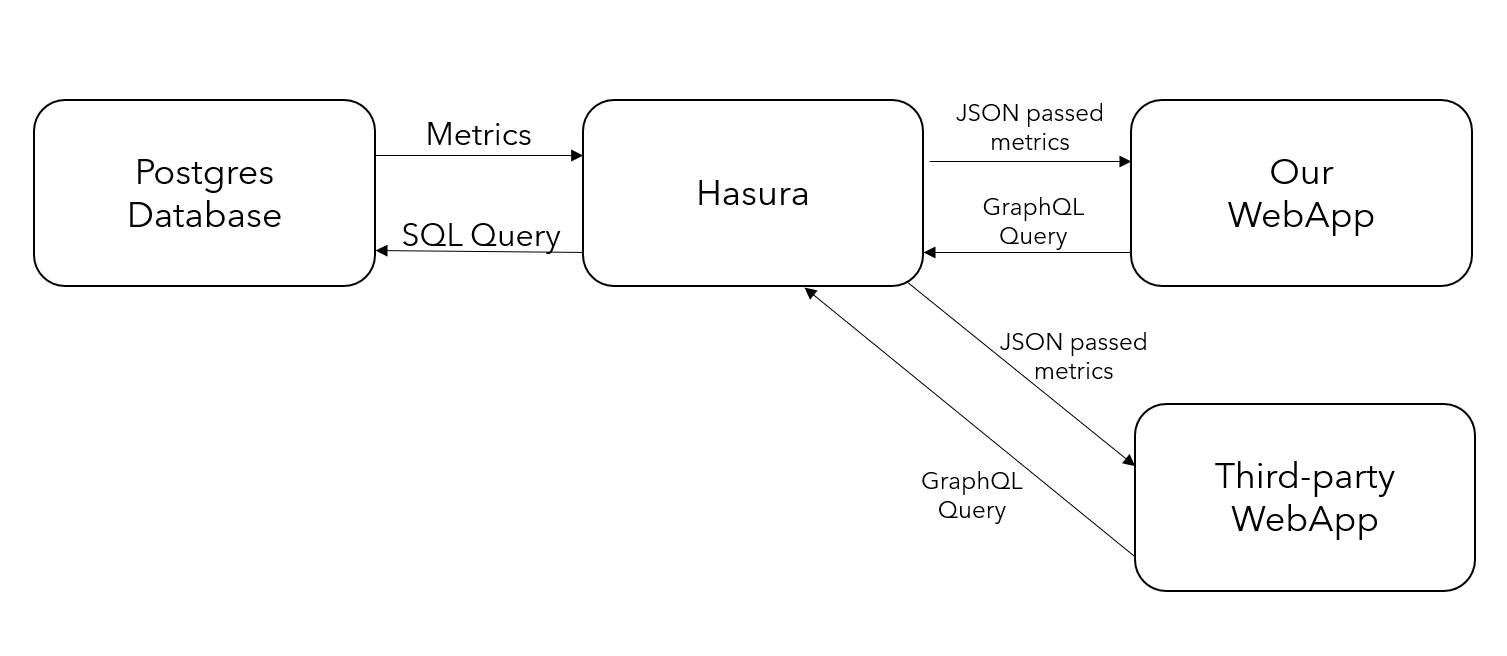
\includegraphics[width=0.80\textwidth]{./img/docker.png}
    \caption{This is a graphical rappresentations of out docker containers and a possible third-party application with their communication}
    \label{fig:docker}
\end{figure}
